\section{Metodologia}

Esta pesquisa tem como objetivo desenvolver uma aplicação web interativa que caracterize e apresente as empresas de Tecnologia da Informação do município de Contagem a partir da integração de dados abertos.
Para isso, bases públicas sobre os estabelecimentos, suas atividades econômicas e seus endereços são coletadas, tratadas e combinadas em um banco de dados único.
Esse banco alimenta uma aplicação com mapa, gráficos, tabelas e filtros, cuja usabilidade é avaliada por inspeção heurística.

\subsection{Objeto de estudo e recorte}

O objeto de estudo são os estabelecimentos de Tecnologia da Informação situados no município de Contagem (MG), identificados pelo código IBGE 3118601.
O setor fica delimitado pela CNAE-Subclasses 2.3 \cite{ibge2020}, só com a atividade principal na divisão 62.
Os códigos incluídos são:

\begin{itemize}
    \item 6201-5/01, desenvolvimento de programas de computador sob encomenda;
    \item 6201-5/02, web design;
    \item 6202-3/00, desenvolvimento e licenciamento de programas de computador customizáveis;
    \item 6203-1/00, desenvolvimento e licenciamento de programas de computador não customizáveis;
    \item 6204-0/00, consultoria em tecnologia da informação;
    \item 6209-1/00, suporte técnico, manutenção e outros serviços em tecnologia da informação.
\end{itemize}

Ficam de fora, neste recorte, hospedagem e portais (divisão 63), comércio e fabricação de equipamentos de informática, conserto de computador e curso de informática.
A unidade de análise é o estabelecimento do cadastro de CNPJ.
Matriz e filial entram como registros distintos quando estiverem no município e na atividade selecionada.
Serão considerados estabelecimentos com situação cadastral ativa na fotografia da base utilizada.
O CNAE secundário não será usado como critério de entrada.

A descrição dos dados será orientada por quatro perguntas: onde esses estabelecimentos se concentram em Contagem; qual é o perfil de porte; qual é a proporção de microempreendedores individuais; e qual parte dos endereços recebe coordenada em cada nível de junção.

Não haverá teste com usuários nem questionário.
A avaliação da interface será uma inspeção feita pelo próprio autor, descrita na Seção \ref{subsec:testes}.
Por isso, não se aplica tramitação em comitê de ética para coleta com pessoas.

\subsection{Proteção de dados}

A base de sócios da Receita Federal, que traz CPF de pessoa física mesmo que mascarado, não será baixada nem carregada na aplicação, porque a unidade de análise é o estabelecimento, e não as pessoas ligadas a ele.
No caso do microempreendedor individual, o nome do estabelecimento pode ser o nome da pessoa; esse nome já é público no cadastro do CNPJ, e a aplicação o exibe como consta ali, sem associá-lo a CPF nem a quadro de sócios.

\subsection{Etapas do trabalho}

Esta pesquisa será realizada em quatro etapas: coleta e tratamento dos dados, desenvolvimento do projeto da solução, implementação da solução e testes.

Na primeira etapa, os estabelecimentos de TI de Contagem são extraídos das bases abertas e integrados em um banco de dados MySQL, com atividade, porte e coordenada.

Na segunda, a aplicação é projetada por meio do levantamento de requisitos, do diagrama de casos de uso e do esquema do banco de dados.

Na terceira, a aplicação é implementada sobre esse banco.

Na quarta, são conferidas a localização atribuída aos estabelecimentos e a usabilidade da interface.

\subsection{Coleta e tratamento dos dados}
\label{subsec:coleta}

A coleta será feita em bases abertas oficiais, por meio do \textit{download} e da consulta aos arquivos publicados por órgãos públicos.

A principal fonte da lista de estabelecimentos será a base pública de CNPJ da Receita Federal do Brasil, que reúne identificação, CNAE, situação cadastral e endereço declarado.
O arquivo de sócios dessa base não será utilizado.

A estrutura e a descrição das atividades virão da CNAE-Subclasses 2.3, mantida pelo IBGE, usada para fechar o recorte da divisão 62.

As coordenadas geográficas serão obtidas no Cadastro Nacional de Endereços para Fins Estatísticos (CNEFE), do IBGE, associado ao Censo Demográfico de 2022.
A base inteira não será geocodificada em lote por serviço online: o CNEFE é a fonte da coordenada.
As malhas territoriais do IBGE fornecerão o contorno do município e, quando disponíveis no nível adequado, recortes internos úteis à agregação espacial, com a área em quilômetros quadrados para a medida relativa.

Para a conferência dos totais, serão consultadas tabelas do Cadastro Central de Empresas (CEMPRE) por meio do SIDRA, sempre no município de Contagem e em nível de CNAE compatível com o recorte.

Como apoio à extração, poderá ser utilizada a plataforma Base dos Dados, desde que os filtros reproduzam o mesmo universo da fonte oficial.

Os arquivos nacionais não serão carregados integralmente na aplicação.
O tratamento ocorrerá em ambiente local, em um banco MySQL de trabalho: os arquivos são importados para tabelas de carga, e a filtragem para Contagem e para as subclasses da divisão 62 é feita em SQL, antes de qualquer junção.

A integração seguirá chaves explícitas: código de município da Receita para isolar Contagem; CNPJ básico para unir estabelecimentos e dados da empresa, como razão social, porte e capital social; CNAE sem máscara para padronizar a atividade; código IBGE 3118601 para ligar o resultado às malhas, ao CNEFE e ao CEMPRE.

O endereço passa por uma padronização antes da junção com o CNEFE.
O CEP fica com 8 dígitos, sem hífen.
O texto vai para maiúsculas, sem acento.
Abreviações comuns de tipo de logradouro são expandidas, como R.\ para RUA e AV.\ para AVENIDA, nos dois lados da junção.
Número vazio ou registrado como S/N não entra na tentativa mais específica.

A junção com o CNEFE segue uma ordem.
Primeiro, tenta-se CEP, logradouro padronizado e número.
Se não houver correspondência, tenta-se só o CEP, e o ponto é marcado como aproximado.
Se o CEP do CNPJ não existir no CNEFE, o estabelecimento continua na base para as contagens e as tabelas, mas fica de fora do mapa de pontos.
Cada registro guarda o nível obtido: endereço completo, só CEP ou sem coordenada.
Com isso, calcula-se a taxa de acerto de cada nível.

O registro também guarda o nível de geocodificação informado pelo próprio CNEFE, na variável \texttt{NV\_GEO\_COORD}.
Esse campo indica se a coordenada é a original do Censo 2022, se foi modificada para apartamentos no mesmo número, se foi estimada pelo IBGE ou se foi atribuída por face de quadra, localidade ou setor censitário.
Assim, uma junção por endereço completo que herdou uma coordenada estimada pelo IBGE não é contada como ponto coletado em campo.

Quando várias empresas recebem a mesma coordenada, o que é esperado no nível de CEP, essa sobreposição fica registrada.
Assim, um CEP com muitas empresas não é tratado como um único endereço conferido no terreno.

O resultado dessa integração será gravado no banco de dados da aplicação, com a data da fotografia das bases.
A aplicação consulta esse banco, e não os arquivos nacionais nem os sites da Receita e do IBGE.

\subsection{Aplicação desenvolvida}

Esta seção apresenta os requisitos da aplicação, a arquitetura da solução, o diagrama de casos de uso e o esquema do banco de dados.

Os requisitos funcionais previstos são:

\begin{itemize}
    \item RF01: exibir um \textit{dashboard} (painel interativo de indicadores) com os indicadores gerais, como o total de estabelecimentos ativos, a distribuição por subclasse da CNAE, o porte e a proporção de microempreendedores individuais;
    \item RF02: filtrar os estabelecimentos por subclasse da CNAE, porte, condição de microempreendedor individual e área do município;
    \item RF03: exibir os estabelecimentos em um mapa de pontos, indicando quantos estão em uma mesma coordenada;
    \item RF04: exibir a quantidade de estabelecimentos por área do município, em total e por quilômetro quadrado;
    \item RF05: listar os estabelecimentos em uma tabela com busca por nome, com CNAE, porte, situação cadastral e endereço;
    \item RF06: informar a data da fotografia das bases e o nível de coordenada de cada estabelecimento.
\end{itemize}

Os requisitos não funcionais previstos são:

\begin{itemize}
    \item RNF01: acesso pelo navegador, sem cadastro de usuário;
    \item RNF02: não exibir CPF, quadro de sócios, telefone ou e-mail;
    \item RNF03: o \textit{dashboard} deve ser integrado, isto é, indicadores, gráficos, mapa e tabela devem responder aos mesmos filtros, sobre os mesmos registros;
    \item RNF04: as consultas devem ser feitas no banco de dados da aplicação, sem depender de serviço externo além do mapa de fundo.
\end{itemize}

A solução será uma aplicação web com arquitetura cliente/servidor, organizada em três partes: os programas de carga, o banco de dados e a aplicação web.
Os programas de carga serão escritos em Python e importarão os arquivos da Receita Federal e do IBGE para tabelas de carga em um banco de dados MySQL, no qual os filtros e as junções descritos na Seção \ref{subsec:coleta} são executados em SQL e gravados nas tabelas finais da aplicação.
O MySQL é usado em todas as etapas, do tratamento dos arquivos à consulta pela aplicação, o que mantém um único sistema de banco de dados no projeto.
A aplicação web será desenvolvida com o SvelteKit, \textit{framework} baseado em JavaScript que reúne a interface executada no navegador, do lado do cliente, e o \textit{back-end} executado no servidor, que consulta o MySQL e entrega à interface os dados já filtrados.
O mapa interativo usará a biblioteca Leaflet, com \textit{tiles} do OpenStreetMap como mapa de fundo.
Uma atualização dos dados será uma nova carga, com outra data de fotografia, e não uma consulta ao vivo às bases da Receita e do IBGE na hora em que alguém abre o site.

A Figura \ref{fig:casos-de-uso} apresenta o diagrama de casos de uso da aplicação, com dois atores.
O visitante consulta os indicadores, aplica filtros, explora o mapa, consulta os estabelecimentos por área e na tabela e vê a data da fotografia e o nível de coordenada.
O administrador, papel exercido pelo autor, carrega uma nova fotografia das bases.

% Diagrama de casos de uso — incluído em textos.tex por % Diagrama de casos de uso — incluído em textos.tex por % Diagrama de casos de uso — incluído em textos.tex por \input{figuras/casos-de-uso}
% Requer no preâmbulo de principal.tex: \usetikzlibrary{shapes,positioning}
\begin{figure}[H]
    \centering
    \caption{Diagrama de casos de uso da aplicação}
    \label{fig:casos-de-uso}
    \vspace{-0.2cm}
    \begin{tikzpicture}[
        caso/.style={
            draw=black,
            thick,
            ellipse,
            font=\small,
            inner sep=0pt,
            minimum height=0.9cm
        },
        assoc/.style={thick},
        ator/.pic={
            \draw[thick] (0,1.05) circle (0.2);
            \draw[thick] (0,0.85) -- (0,0.3);
            \draw[thick] (-0.35,0.65) -- (0.35,0.65);
            \draw[thick] (0,0.3) -- (-0.3,-0.15);
            \draw[thick] (0,0.3) -- (0.3,-0.15);
        }
    ]
        \draw[thick] (-3.9,4.0) rectangle (3.9,-4.9);
        \node[font=\small\bfseries, anchor=north] at (0,3.95) {Aplicação web};

        \node[caso] (uc1) at (0,2.9) {Consultar indicadores gerais};
        \node[caso] (uc2) at (0,1.7) {Filtrar estabelecimentos};
        \node[caso] (uc3) at (0,0.5) {Explorar o mapa de pontos};
        \node[caso] (uc4) at (0,-0.7) {Consultar densidade por área};
        \node[caso] (uc5) at (0,-1.9) {Buscar na tabela por nome};
        \node[caso] (uc6) at (0,-3.1) {Ver data e nível de coordenada};
        \node[caso] (uc7) at (0,-4.3) {Carregar nova fotografia};

        \pic at (-5.8,-0.6) {ator};
        \node[font=\small, below] at (-5.8,-0.75) {Visitante};
        \coordinate (v) at (-5.4,0.35);
        \foreach \uc in {uc1,uc2,uc3,uc4,uc5,uc6} {
            \draw[assoc] (v) -- (\uc.west);
        }

        \pic at (5.8,-4.9) {ator};
        \node[font=\small, below] at (5.8,-5.05) {Administrador};
        \draw[assoc] (5.4,-4.15) -- (uc7.east);
    \end{tikzpicture}
    \vspace{-0.2cm}
    \\\textbf{\footnotesize Fonte: Elaborado pelo autor.}
\end{figure}

% Requer no preâmbulo de principal.tex: \usetikzlibrary{shapes,positioning}
\begin{figure}[H]
    \centering
    \caption{Diagrama de casos de uso da aplicação}
    \label{fig:casos-de-uso}
    \vspace{-0.2cm}
    \begin{tikzpicture}[
        caso/.style={
            draw=black,
            thick,
            ellipse,
            font=\small,
            inner sep=0pt,
            minimum height=0.9cm
        },
        assoc/.style={thick},
        ator/.pic={
            \draw[thick] (0,1.05) circle (0.2);
            \draw[thick] (0,0.85) -- (0,0.3);
            \draw[thick] (-0.35,0.65) -- (0.35,0.65);
            \draw[thick] (0,0.3) -- (-0.3,-0.15);
            \draw[thick] (0,0.3) -- (0.3,-0.15);
        }
    ]
        \draw[thick] (-3.9,4.0) rectangle (3.9,-4.9);
        \node[font=\small\bfseries, anchor=north] at (0,3.95) {Aplicação web};

        \node[caso] (uc1) at (0,2.9) {Consultar indicadores gerais};
        \node[caso] (uc2) at (0,1.7) {Filtrar estabelecimentos};
        \node[caso] (uc3) at (0,0.5) {Explorar o mapa de pontos};
        \node[caso] (uc4) at (0,-0.7) {Consultar densidade por área};
        \node[caso] (uc5) at (0,-1.9) {Buscar na tabela por nome};
        \node[caso] (uc6) at (0,-3.1) {Ver data e nível de coordenada};
        \node[caso] (uc7) at (0,-4.3) {Carregar nova fotografia};

        \pic at (-5.8,-0.6) {ator};
        \node[font=\small, below] at (-5.8,-0.75) {Visitante};
        \coordinate (v) at (-5.4,0.35);
        \foreach \uc in {uc1,uc2,uc3,uc4,uc5,uc6} {
            \draw[assoc] (v) -- (\uc.west);
        }

        \pic at (5.8,-4.9) {ator};
        \node[font=\small, below] at (5.8,-5.05) {Administrador};
        \draw[assoc] (5.4,-4.15) -- (uc7.east);
    \end{tikzpicture}
    \vspace{-0.2cm}
    \\\textbf{\footnotesize Fonte: Elaborado pelo autor.}
\end{figure}

% Requer no preâmbulo de principal.tex: \usetikzlibrary{shapes,positioning}
\begin{figure}[H]
    \centering
    \caption{Diagrama de casos de uso da aplicação}
    \label{fig:casos-de-uso}
    \vspace{-0.2cm}
    \begin{tikzpicture}[
        caso/.style={
            draw=black,
            thick,
            ellipse,
            font=\small,
            inner sep=0pt,
            minimum height=0.9cm
        },
        assoc/.style={thick},
        ator/.pic={
            \draw[thick] (0,1.05) circle (0.2);
            \draw[thick] (0,0.85) -- (0,0.3);
            \draw[thick] (-0.35,0.65) -- (0.35,0.65);
            \draw[thick] (0,0.3) -- (-0.3,-0.15);
            \draw[thick] (0,0.3) -- (0.3,-0.15);
        }
    ]
        \draw[thick] (-3.9,4.0) rectangle (3.9,-4.9);
        \node[font=\small\bfseries, anchor=north] at (0,3.95) {Aplicação web};

        \node[caso] (uc1) at (0,2.9) {Consultar indicadores gerais};
        \node[caso] (uc2) at (0,1.7) {Filtrar estabelecimentos};
        \node[caso] (uc3) at (0,0.5) {Explorar o mapa de pontos};
        \node[caso] (uc4) at (0,-0.7) {Consultar densidade por área};
        \node[caso] (uc5) at (0,-1.9) {Buscar na tabela por nome};
        \node[caso] (uc6) at (0,-3.1) {Ver data e nível de coordenada};
        \node[caso] (uc7) at (0,-4.3) {Carregar nova fotografia};

        \pic at (-5.8,-0.6) {ator};
        \node[font=\small, below] at (-5.8,-0.75) {Visitante};
        \coordinate (v) at (-5.4,0.35);
        \foreach \uc in {uc1,uc2,uc3,uc4,uc5,uc6} {
            \draw[assoc] (v) -- (\uc.west);
        }

        \pic at (5.8,-4.9) {ator};
        \node[font=\small, below] at (5.8,-5.05) {Administrador};
        \draw[assoc] (5.4,-4.15) -- (uc7.east);
    \end{tikzpicture}
    \vspace{-0.2cm}
    \\\textbf{\footnotesize Fonte: Elaborado pelo autor.}
\end{figure}


A Figura \ref{fig:esquema-banco} apresenta o esquema do banco de dados MySQL.
Cada estabelecimento se liga à empresa pelo CNPJ básico, à atividade pela subclasse da CNAE e à carga em que foi gravado.
A localização guarda a coordenada, o nível de junção com o CNEFE, o nível de geocodificação informado pelo próprio CNEFE e a área do município em que o ponto está.
A carga registra a data da fotografia, as versões das bases, a data de \textit{download} e as regras de filtro, para que o processo possa ser refeito.

% Esquema do banco de dados MySQL — incluído em o_software_desenvolvido.tex ou metodologia.tex por % Esquema do banco de dados MySQL — incluído em o_software_desenvolvido.tex ou metodologia.tex por % Esquema do banco de dados MySQL — incluído em o_software_desenvolvido.tex ou metodologia.tex por \input{figuras/esquema-banco}
% Requer no preâmbulo de principal.tex: \usetikzlibrary{positioning}
% Reflete o esquema gerado por pipeline_para_obtencao_de_dados/sql_gerado/schema_aplicacao.sql
\begin{figure}[H]
    \centering
    \caption{Esquema do banco de dados da aplicação}
    \label{fig:esquema-banco}
    \vspace{-0.2cm}
    \renewcommand{\arraystretch}{1.05}
    \begin{adjustbox}{scale=0.85}
    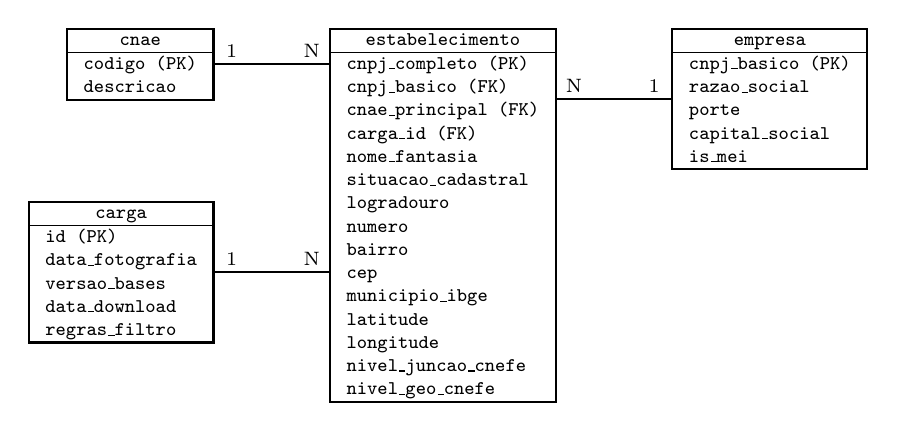
\begin{tikzpicture}[
        tabela/.style={
            draw=black,
            thick,
            inner sep=0pt,
            font=\scriptsize\ttfamily,
            fill=white
        },
        rel/.style={thick},
        card/.style={font=\scriptsize, inner sep=2pt}
    ]
        \node[tabela, anchor=north] (estab) at (0,0) {%
            \begin{tabular}{l}
                \multicolumn{1}{c}{\textbf{estabelecimento}} \\ \hline
                cnpj\_completo (PK) \\
                cnpj\_basico (FK) \\
                cnae\_principal (FK) \\
                carga\_id (FK) \\
                nome\_fantasia \\
                situacao\_cadastral \\
                logradouro \\
                numero \\
                bairro \\
                cep \\
                municipio\_ibge \\
                latitude \\
                longitude \\
                nivel\_juncao\_cnefe \\
                nivel\_geo\_cnefe
            \end{tabular}};

        \node[tabela, anchor=north east] (cnae) at (-2.9,0) {%
            \begin{tabular}{l}
                \multicolumn{1}{c}{\textbf{cnae}} \\ \hline
                codigo (PK) \\
                descricao
            \end{tabular}};

        \node[tabela, anchor=north west] (empresa) at (2.9,0) {%
            \begin{tabular}{l}
                \multicolumn{1}{c}{\textbf{empresa}} \\ \hline
                cnpj\_basico (PK) \\
                razao\_social \\
                porte \\
                capital\_social \\
                is\_mei
            \end{tabular}};

        \node[tabela, anchor=north east] (carga) at (-2.9,-2.2) {%
            \begin{tabular}{l}
                \multicolumn{1}{c}{\textbf{carga}} \\ \hline
                id (PK) \\
                data\_fotografia \\
                versao\_bases \\
                data\_download \\
                regras\_filtro
            \end{tabular}};

        \draw[rel] (cnae.east) -- node[card, pos=0.15, above] {1} node[card, pos=0.85, above] {N} (cnae.east -| estab.west);
        \draw[rel] (empresa.west) -- node[card, pos=0.15, above] {1} node[card, pos=0.85, above] {N} (empresa.west -| estab.east);
        \draw[rel] (carga.east) -- node[card, pos=0.15, above] {1} node[card, pos=0.85, above] {N} (carga.east -| estab.west);
    \end{tikzpicture}
    \end{adjustbox}
    \vspace{-0.2cm}
    \\\textbf{\footnotesize Fonte: Elaborado pelo autor.}
\end{figure}

% Requer no preâmbulo de principal.tex: \usetikzlibrary{positioning}
% Reflete o esquema gerado por pipeline_para_obtencao_de_dados/sql_gerado/schema_aplicacao.sql
\begin{figure}[H]
    \centering
    \caption{Esquema do banco de dados da aplicação}
    \label{fig:esquema-banco}
    \vspace{-0.2cm}
    \renewcommand{\arraystretch}{1.05}
    \begin{adjustbox}{scale=0.85}
    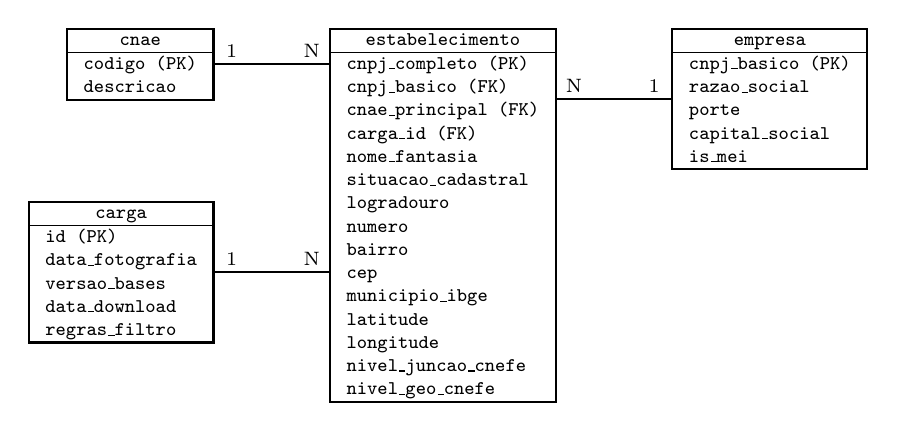
\begin{tikzpicture}[
        tabela/.style={
            draw=black,
            thick,
            inner sep=0pt,
            font=\scriptsize\ttfamily,
            fill=white
        },
        rel/.style={thick},
        card/.style={font=\scriptsize, inner sep=2pt}
    ]
        \node[tabela, anchor=north] (estab) at (0,0) {%
            \begin{tabular}{l}
                \multicolumn{1}{c}{\textbf{estabelecimento}} \\ \hline
                cnpj\_completo (PK) \\
                cnpj\_basico (FK) \\
                cnae\_principal (FK) \\
                carga\_id (FK) \\
                nome\_fantasia \\
                situacao\_cadastral \\
                logradouro \\
                numero \\
                bairro \\
                cep \\
                municipio\_ibge \\
                latitude \\
                longitude \\
                nivel\_juncao\_cnefe \\
                nivel\_geo\_cnefe
            \end{tabular}};

        \node[tabela, anchor=north east] (cnae) at (-2.9,0) {%
            \begin{tabular}{l}
                \multicolumn{1}{c}{\textbf{cnae}} \\ \hline
                codigo (PK) \\
                descricao
            \end{tabular}};

        \node[tabela, anchor=north west] (empresa) at (2.9,0) {%
            \begin{tabular}{l}
                \multicolumn{1}{c}{\textbf{empresa}} \\ \hline
                cnpj\_basico (PK) \\
                razao\_social \\
                porte \\
                capital\_social \\
                is\_mei
            \end{tabular}};

        \node[tabela, anchor=north east] (carga) at (-2.9,-2.2) {%
            \begin{tabular}{l}
                \multicolumn{1}{c}{\textbf{carga}} \\ \hline
                id (PK) \\
                data\_fotografia \\
                versao\_bases \\
                data\_download \\
                regras\_filtro
            \end{tabular}};

        \draw[rel] (cnae.east) -- node[card, pos=0.15, above] {1} node[card, pos=0.85, above] {N} (cnae.east -| estab.west);
        \draw[rel] (empresa.west) -- node[card, pos=0.15, above] {1} node[card, pos=0.85, above] {N} (empresa.west -| estab.east);
        \draw[rel] (carga.east) -- node[card, pos=0.15, above] {1} node[card, pos=0.85, above] {N} (carga.east -| estab.west);
    \end{tikzpicture}
    \end{adjustbox}
    \vspace{-0.2cm}
    \\\textbf{\footnotesize Fonte: Elaborado pelo autor.}
\end{figure}

% Requer no preâmbulo de principal.tex: \usetikzlibrary{positioning}
% Reflete o esquema gerado por pipeline_para_obtencao_de_dados/sql_gerado/schema_aplicacao.sql
\begin{figure}[H]
    \centering
    \caption{Esquema do banco de dados da aplicação}
    \label{fig:esquema-banco}
    \vspace{-0.2cm}
    \renewcommand{\arraystretch}{1.05}
    \begin{adjustbox}{scale=0.85}
    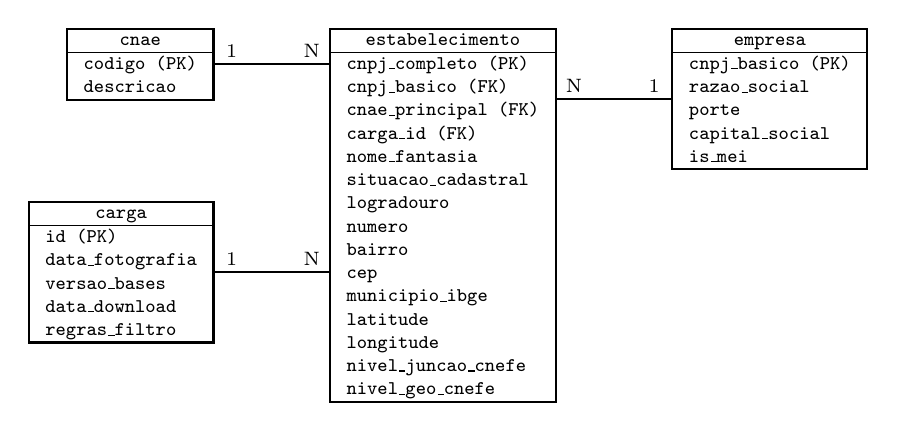
\begin{tikzpicture}[
        tabela/.style={
            draw=black,
            thick,
            inner sep=0pt,
            font=\scriptsize\ttfamily,
            fill=white
        },
        rel/.style={thick},
        card/.style={font=\scriptsize, inner sep=2pt}
    ]
        \node[tabela, anchor=north] (estab) at (0,0) {%
            \begin{tabular}{l}
                \multicolumn{1}{c}{\textbf{estabelecimento}} \\ \hline
                cnpj\_completo (PK) \\
                cnpj\_basico (FK) \\
                cnae\_principal (FK) \\
                carga\_id (FK) \\
                nome\_fantasia \\
                situacao\_cadastral \\
                logradouro \\
                numero \\
                bairro \\
                cep \\
                municipio\_ibge \\
                latitude \\
                longitude \\
                nivel\_juncao\_cnefe \\
                nivel\_geo\_cnefe
            \end{tabular}};

        \node[tabela, anchor=north east] (cnae) at (-2.9,0) {%
            \begin{tabular}{l}
                \multicolumn{1}{c}{\textbf{cnae}} \\ \hline
                codigo (PK) \\
                descricao
            \end{tabular}};

        \node[tabela, anchor=north west] (empresa) at (2.9,0) {%
            \begin{tabular}{l}
                \multicolumn{1}{c}{\textbf{empresa}} \\ \hline
                cnpj\_basico (PK) \\
                razao\_social \\
                porte \\
                capital\_social \\
                is\_mei
            \end{tabular}};

        \node[tabela, anchor=north east] (carga) at (-2.9,-2.2) {%
            \begin{tabular}{l}
                \multicolumn{1}{c}{\textbf{carga}} \\ \hline
                id (PK) \\
                data\_fotografia \\
                versao\_bases \\
                data\_download \\
                regras\_filtro
            \end{tabular}};

        \draw[rel] (cnae.east) -- node[card, pos=0.15, above] {1} node[card, pos=0.85, above] {N} (cnae.east -| estab.west);
        \draw[rel] (empresa.west) -- node[card, pos=0.15, above] {1} node[card, pos=0.85, above] {N} (empresa.west -| estab.east);
        \draw[rel] (carga.east) -- node[card, pos=0.15, above] {1} node[card, pos=0.85, above] {N} (carga.east -| estab.west);
    \end{tikzpicture}
    \end{adjustbox}
    \vspace{-0.2cm}
    \\\textbf{\footnotesize Fonte: Elaborado pelo autor.}
\end{figure}


\subsection{Testes}
\label{subsec:testes}

Os testes verificam dois aspectos da aplicação: a localização atribuída aos estabelecimentos e a usabilidade da interface.

Para estimar o erro da localização, uma amostra de cerca de 30 endereços será conferida em outra fonte, por consulta manual no mapa ou por um serviço de geocodificação usado só nessa amostra.
A conferência não substitui o CNEFE na base inteira.
Ela serve para dizer, de forma aproximada, o quanto o ponto se afasta do endereço informado.

Os totais da base também serão comparados com os do CEMPRE.
A comparação não busca números iguais, porque o ano e os critérios de cada base são diferentes.
O que se verifica é se a ordem de grandeza é coerente.

A usabilidade será avaliada por inspeção heurística, feita pelo autor, sem usuários convidados.
A lista usada é a das dez heurísticas de \citeonline{nielsen1994}, no mesmo tipo de registro adotado por \citeonline{vazquezingelmo2024}: problema encontrado, heurística relacionada e gravidade.
A gravidade será anotada em três níveis: leve, médio e grave.
As telas percorridas serão o mapa, os filtros, os gráficos e a tabela.
O resultado dessa inspeção entra na seção de resultados, como lista de problemas e ajustes possíveis, e não como nota da aplicação.

\subsection{Procedimentos de análise}

A análise será descritiva e seguirá as quatro perguntas do objeto de estudo.
Serão calculados totais de estabelecimentos ativos no recorte, a distribuição por subclasse da CNAE, o perfil de porte e a proporção de microempreendedores individuais.
Também serão apresentados os percentuais de georreferenciamento em cada nível de junção.

No mapa, serão observados onde os pontos se concentram, onde há vazios e como os estabelecimentos se distribuem pelos recortes territoriais disponíveis.
A comparação entre áreas usa o total e uma medida normalizada, o número de estabelecimentos por quilômetro quadrado, para uma área maior não parecer mais concentrada só por ter mais espaço.
Mapas de pontos e, quando a taxa de coordenada permitir, uma representação de densidade ajudam essa leitura, com o aviso sobre pontos sobrepostos.

Os resultados serão apresentados em tabelas, gráficos e mapas, e discutidos na seção de resultados.
